\documentclass[tikz,border=6pt]{standalone}
\usepackage[T1]{fontenc}
\usepackage{helvet}
\renewcommand{\familydefault}{\sfdefault}
\usepackage{tikz}
\usetikzlibrary{positioning}

\definecolor{ink}{HTML}{1F2937}
\definecolor{muted}{HTML}{6B7280}
\definecolor{head}{HTML}{1E3A5F}
\definecolor{prov}{HTML}{1D4ED8}
\definecolor{provbg}{HTML}{EFF6FF}
\definecolor{enc}{HTML}{047857}
\definecolor{encbg}{HTML}{ECFDF5}
\definecolor{ssl}{HTML}{C2410C}
\definecolor{sslbg}{HTML}{FFF7ED}
\definecolor{chip}{HTML}{F8FAFC}

\begin{document}
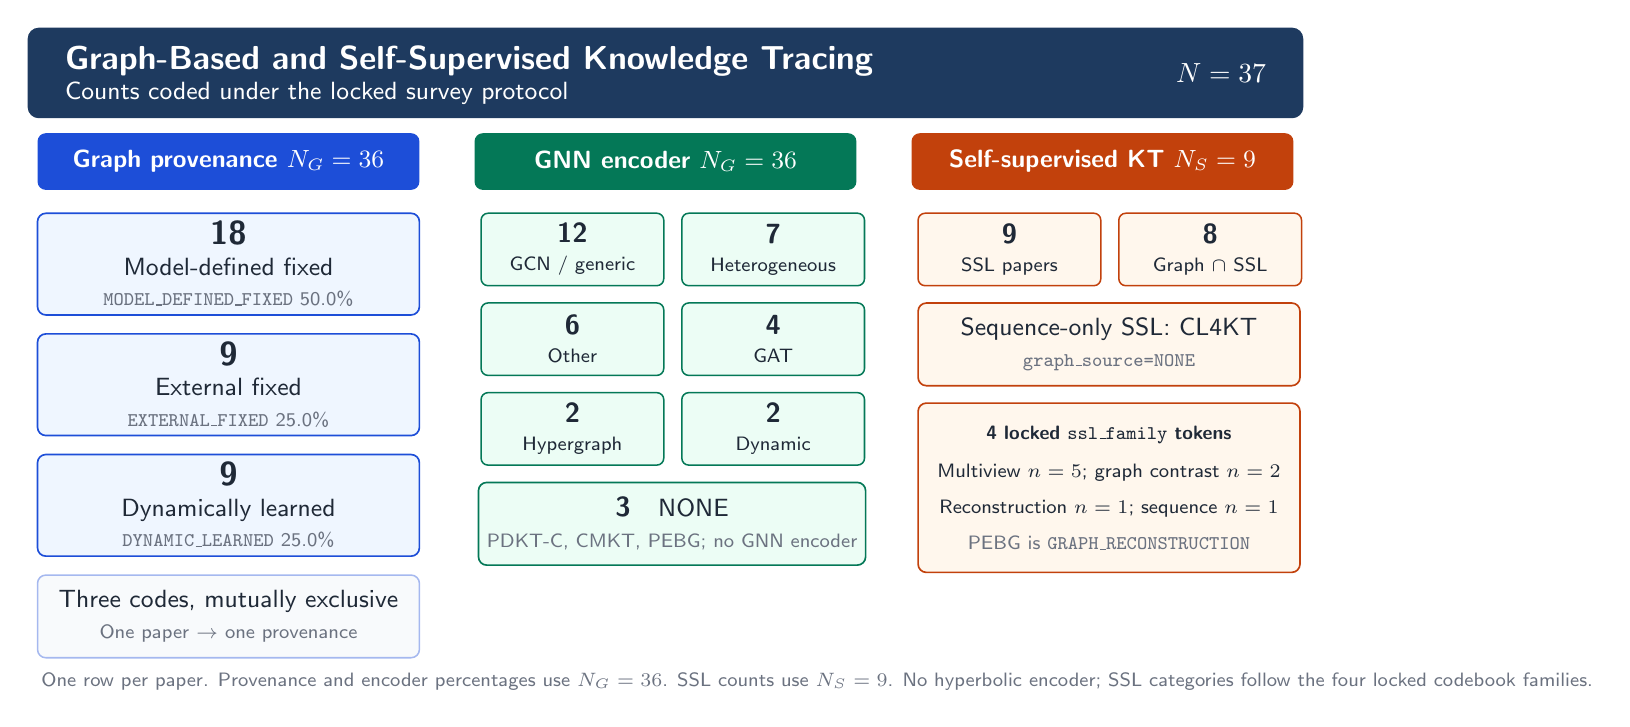
\begin{tikzpicture}[font=\sffamily]

\tikzset{
  pcard/.style={rectangle, rounded corners=3pt, align=center,
    minimum width=4.85cm, minimum height=1.05cm, inner sep=3pt,
    draw=prov, fill=provbg, line width=0.6pt, text=ink},
  pnote/.style={rectangle, rounded corners=3pt, align=center,
    minimum width=4.85cm, minimum height=1.05cm, inner sep=3pt,
    draw=prov!40, fill=chip, line width=0.55pt, text=ink},
  echip/.style={rectangle, rounded corners=2.5pt, align=center,
    minimum width=2.32cm, minimum height=0.92cm, inner sep=2pt,
    draw=enc, fill=encbg, line width=0.55pt, text=ink},
  ecard/.style={rectangle, rounded corners=3pt, align=center,
    minimum width=4.85cm, minimum height=1.05cm, inner sep=3pt,
    draw=enc, fill=encbg, line width=0.6pt, text=ink},
  schip/.style={rectangle, rounded corners=2.5pt, align=center,
    minimum width=2.32cm, minimum height=0.92cm, inner sep=2pt,
    draw=ssl, fill=sslbg, line width=0.55pt, text=ink},
  scard/.style={rectangle, rounded corners=3pt, align=center,
    minimum width=4.85cm, inner sep=3pt,
    draw=ssl, fill=sslbg, line width=0.6pt, text=ink},
  colh/.style={rectangle, rounded corners=3pt, align=center,
    minimum width=4.85cm, minimum height=0.72cm, text=white,
    font=\sffamily\bfseries\small}
}

\fill[head, rounded corners=4pt] (0,0) rectangle (16.2,1.15);
\node[anchor=west, text=white, font=\sffamily\bfseries\large] at (0.35,0.72)
  {Graph-Based~and~Self-Supervised~Knowledge~Tracing};
\node[anchor=west, text=white!88, font=\sffamily\small] at (0.35,0.32)
  {Counts coded under the locked survey protocol};
\node[anchor=east, text=white, font=\sffamily\bfseries] at (15.85,0.58) {$N=37$};

\node[colh, fill=prov] (h1) at (2.55,-0.55) {Graph provenance  $N_G=36$};
\node[colh, fill=enc]  (h2) at (8.10,-0.55) {GNN encoder  $N_G=36$};
\node[colh, fill=ssl]  (h3) at (13.65,-0.55) {Self-supervised KT  $N_S=9$};

\node[pcard, below=0.28cm of h1] (p1) {%
  {\fontsize{13}{15}\selectfont\bfseries 18}\\[-1pt]
  {\small Model-defined fixed}\\[-1pt]
  {\scriptsize\color{muted}\texttt{MODEL\_DEFINED\_FIXED}  50.0\%}};
\node[pcard, below=0.22cm of p1] (p2) {%
  {\fontsize{13}{15}\selectfont\bfseries 9}\\[-1pt]
  {\small External fixed}\\[-1pt]
  {\scriptsize\color{muted}\texttt{EXTERNAL\_FIXED}  25.0\%}};
\node[pcard, below=0.22cm of p2] (p3) {%
  {\fontsize{13}{15}\selectfont\bfseries 9}\\[-1pt]
  {\small Dynamically learned}\\[-1pt]
  {\scriptsize\color{muted}\texttt{DYNAMIC\_LEARNED}  25.0\%}};
\node[pnote, below=0.22cm of p3] (p4) {%
  {\small Three codes, mutually exclusive}\\[-1pt]
  {\scriptsize\color{muted}One paper $\rightarrow$ one provenance}};

\node[echip, below left=0.28cm and -2.42cm of h2] (e1) {{\bfseries 12}\\[-2pt]{\scriptsize GCN / generic}};
\node[echip, right=0.21cm of e1] (e2) {{\bfseries 7}\\[-2pt]{\scriptsize Heterogeneous}};
\node[echip, below=0.20cm of e1] (e3) {{\bfseries 6}\\[-2pt]{\scriptsize Other}};
\node[echip, right=0.21cm of e3] (e4) {{\bfseries 4}\\[-2pt]{\scriptsize GAT}};
\node[echip, below=0.20cm of e3] (e5) {{\bfseries 2}\\[-2pt]{\scriptsize Hypergraph}};
\node[echip, right=0.21cm of e5] (e6) {{\bfseries 2}\\[-2pt]{\scriptsize Dynamic}};
\node[ecard, below=0.20cm of e5, xshift=1.265cm] (e7) {%
  {\bfseries 3}\quad{\small NONE}\\[-1pt]
  {\scriptsize\color{muted}PDKT-C, CMKT, PEBG; no GNN encoder}};

\node[schip, below left=0.28cm and -2.42cm of h3] (s1) {{\bfseries 9}\\[-2pt]{\scriptsize SSL papers}};
\node[schip, right=0.21cm of s1] (s2) {{\bfseries 8}\\[-2pt]{\scriptsize Graph $\cap$ SSL}};
\node[scard, minimum height=1.05cm, below=0.20cm of s1, xshift=1.265cm] (s3) {%
  {\small Sequence-only SSL: CL4KT}\\[-1pt]
  {\scriptsize\color{muted}\texttt{graph\_source=NONE}}};
\node[scard, minimum height=2.15cm, below=0.20cm of s3] (s4) {%
  {\scriptsize\bfseries 4 locked \texttt{ssl\_family} tokens}\\[2pt]
  {\scriptsize Multiview $n=5$; graph contrast $n=2$}\\[1pt]
  {\scriptsize Reconstruction $n=1$; sequence $n=1$}\\[1pt]
  {\scriptsize\color{muted}PEBG is \texttt{GRAPH\_RECONSTRUCTION}}};

\node[anchor=west, text=muted, font=\sffamily\scriptsize] at (0.05,-7.15)
  {One row per paper. Provenance and encoder percentages use $N_G=36$. SSL counts use $N_S=9$. No hyperbolic encoder; SSL categories follow the four locked codebook families.};

\end{tikzpicture}
\end{document}
